\documentclass[runningheads]{llncs}

\usepackage{graphicx}
\usepackage{listings}


\begin{document}

% \thanks{Supported by organization x.}
\title{A Study in Cuda Usage}
\author{Pedro Carrega\inst{1} \and
Vasco Ferreira\inst{1}
}
%\authorrunning{F. Author et al.}

\institute{Departamento de Informática da Faculdade de Ciências da Universidade de Lisboa
\email{\{fc49080,fc49070\}@alunos.fc.ul.pt}}

\maketitle

\begin{abstract}
This paper was developed with the purpose to explain GPU programing and the improvements that can be made. To demonstrate this we used the Floyd-Warshall algorithm since it is very demanding for the CPU due to the high number of computations required. During our research we discovered that the available materials for learning GPGPU are quite difficult to understand for those who are looking to learn the basics of GPU programing. For that we developed this paper explaining from scratch GPGPU and some of the most significant improvements that can be made. We will start with a simple sequential solution of the algorithm in CUDA and from there go step by step till we use most of the tools and processing power that a GPU has to offer. This paper is helpful for someone who intends to learn the basics of GPGPU or could be used as a teaching guide in an IT course to introduce GPGPU to students.

\keywords{GPGPU  \and CUDA \and Floyd-Warshall.}
\end{abstract}
%
%
%
\section{Introduction}

The purpose of this paper is to teach the basics of GPGPU programing. 
The usage of GPUs is more and more common 
The introduction should set the context for your project. Why is this topic relevant?

You should also define the scope of your project. You could design a software artifact that would end poverty and famine, but that is not realistic.

For example, this document describes the structure your paper should have. Despite using the LNCS LaTeX template \footnote{LNCS is the official template for Europar 2019, in case you are interested.}, the formatting template is not relevant, only the content structure is relevant.

Finally, you should define the goals of your project. For instance,

\begin{itemize}
	\item To propose a method for the parallelization of Genetic Algorithms
	\item An implementation of such algorithm
	\item The experimental evaluation of such method, with comparison with a sequential alternative.
\end{itemize}


\section{Background}

This is an optional section, as it depends on your project. In projects where a given specific knowledge is required to understand the article, you should give a brief introduction of the required concepts. In the case of genetic algorithms, you should present the basic algorithm in this section.


\section{Approach}

In this section, you should present your approach. Notice that an approach may be different than an implementation. An approach should be generic and ideally applied for different machines, virtual machines or languages. You should present algorithms or generic diagrams explaining the approach.

\section{Implementation Details}

In this section you can talk about details of how you implemented your approach. Depending on the detail of your approach, this might be an optional section.

As an example, I would detail how I implemented the phaser in the genetic algorithm, or how I implemented parallel mergesort on ForkJoin. Another aspect could be how to organize your arrays to minimize overhead in recursive calls.

\section{Versions}
\subsection{Sequential CPU}
In order to demonstrate the effectiveness of the usage of GPGPUs in the processing 
of some problems we started by implementing our problem in the CPU so we could use the results as a reference point to our others solutions.
%nao sei se devia por este paragrafo abaixo

This solution will only use one thread of the CPU as the purpose of this paper is to demonstrate the impact of the improvements that can be made on the GPGPU.
The graph we will be using for the Floyd-Warshall problem will be a two dimensional graph, in another words, a 2D grid.
With that in mind, we by creating 3 \textit{for} cycles each will start at 0 and will iterate a number of times corresponding to the size of the graph.
The second and third cycle will correspond to the X and Y coordinates, respectively, 
while the first cycle will match an intermediate point for which the shortest path will be computed.
%nao sei se meto esta ultima parte.
Inside the last cycle it will be compared the direct distance of X to Y with the addition of the distances 
of X to K and K to Y, in case the latter is smaller the distance of X to Y is updated with the value of the addition.

\subsection{Sequential GPU}
To start our learning of how to program in the GPU we will start by doing the most basic implementation possible, 
one thread computing the entirety of the Floyd-Warshall problem.
GPU functions work like any other CPU functions barring two simple differences. 

First, a GPU function has either the \textit{\_\_global\_\_} or the \textit{\_\_device\_\_} \dots%k usar aqui? tag? keyword?
where \textit{\_\_global\_\_} is a function that will be called by the CPU but run on the GPU 
and \textit{\_\_device\_\_} is a function that is called by the GPU to be run by the GPU. 
This \dots can also be used to initialize a global variable on the GPU.

Second, the syntax of the call of a GPU function also differs. Kernels work on a grid basis, and such, you need to indicate the grid your program will be working on. 
That indication is made by placing
\begin{math} <<< X, Y >>> \end{math}
after the name of the function, where X represents the number of blocks to be used and Y the number of threads to be used per block, respectively. 

Having copied our graph to the GPU memory, we call our kernel with one block and one thread per block, 
Inside our GPU function we apply the same programing logic that was applied for the sequential CPU version of the Floyd-Warshall problem. 
We create 3 \textit{for} cycles to iterate through our graph and compute our problem.


\subsection{Parallel GPU}
Using a single thread to compute a problem on the GPU goes against it's strengths. 
Due to the low core clock speed, the strength of the GPU comes from it's high thread count being able to compute multiple values at the same time. 

When running a function parallel on the GPU each thread will run it's own instance of that same function, 
in other words, the implementation of the function now needs to take into consideration how we partition the work load for each thread. 
Having decided the number of threads per blocks we want to use, the most common way to split the work load is to 
use that number to divide the size of our problem, this way obtaining the number of blocks we are going to use to compute our problem. 

Obviously we are going to follow that same logic, but seeing that our problem uses a 2D grid, 
applying a 2D grid to our blocks and threads. Such can be made using \textit{dim3()} \dots, 
and so our kernel call will look like: \newline\small{\textit{parallelGPU}
\begin{math} <<< \end{math}
\textit{dim3(GRAPH\_SIZE/NThreads,GRAPH\_SIZE/NThreads),\newline dim3(NThreads,NThreads)}
\begin{math} >>> \end{math}}. \newline
Where GRAPH\_Size is the size of our graph and NThreads the number of threads we decided to use.

Regarding the implementation of our function, we have to change it completely.
The kernel is now called K times by the CPU, where K goes from 0 to GRAPH\_SIZE, 
each thread will now be attributed two coordinates determined by their coordinates in the 2D grid. 
If the coordinates are withing the scope of the problem they will try to compute the shortest path between X to Y, using the value of K provided by the CPU when the kernel is called, updating the value if needed. 
%In order to improve performance, to the values of X and Y are added the block dimension multiplied by the dimension of the grid. After, if the coordinates are still within the scope of the problem, the thread will compute again using the new coordinates.%compute? 

\subsection{Work Load}

How we partition the work load for each thread may have a big impact on the performance of our solution. Like mentioned before, the major strength of the GPU is it's high thread count so that it can compute multiple values at the same time.
During our research into the topic we came up with the following guidelines in order to optimize work load: %algo me melhor k "came up with"
\begin{enumerate}
	\item Every thread works the same amount
	\item Use the most amount of threads possible
	\item Avoid using the scheduler
	\newline
\end{enumerate}
%nao gosto deste paragrafo
1. Considering every thread follows the program counter of the block, meaning the thread is only allowed to compute a certain line when the block allows it.
Threads with less work load might find themselves in a situation where they must sit idle waiting for others threads to catch up.
This scenario is avoided by a correct split of the work load, making every thread in the same block be synchronized on the computation it needs to execute.
\newline
\newline
%e deste
2. Simply put, the more threads you have available to compute your problem the more you can divide your problem. A major cavite however is to not use more threads than those that are available on the GPU. When the number of threads used is bigger than those available the GPU scheduler begins to be involved a major overhead is added to the computation cutting a lot of the performance offered by the GPU.
\newline
\newline
%ja disse k nao tou inspirado hj?
3. Like mentioned before, using the GPU scheduler adds a major overhead to the computation, so it makes sense we try to avoid using it.
One possible workaround, on a kernel call that uses loops and the problem is bigger than the number of threads offered by the GPU, is to increment the value of the coordinates variable by the product of the dimension of the block by the dimension of the grid. Doing this

To use the major strength of the GPU we have to decide how to partition the work each thread will do. 
Ideally we would use the lowest number of blocks possible, allowing use of shared memory and block synchronization, but we getting ahead of ourselves %use this cheeky line? 
To show the importance of using a correct work load we will implement

\subsection{Synchronization}


\subsection{Shared Memory}


\section{Evaluation}

\subsection{Experimental Setup}

In this section you should describe the machine(s) in which you are going to evaluate your system. Select the information that is relevant.


\subsection{Results}

In this section you should present the results. Do not forget to explain where the data came from. 

You should include (ideally vectorial) plots, with a descriptive caption. Make sure all the plots (Like Figure~\ref{fig1} are well identified and axis and metrics are defined.

\begin{figure}[htbp]
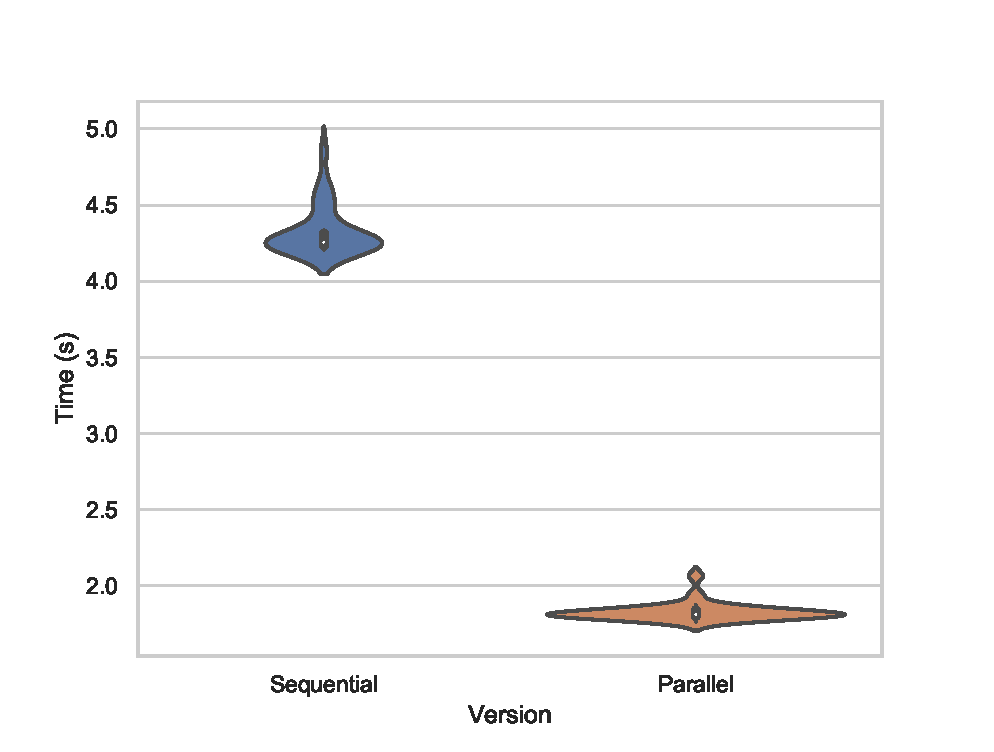
\includegraphics[width=\textwidth]{code/performance.eps}
\caption{Comparison of the performance of sequential and parallel versions of the algorithm.} \label{fig1}
\end{figure}


\subsection{Discussion}

Here you should discuss the results on a high level. For instance, based on our results, the parallelization of the merge-sort is relevant as no other parallel work occurs at the same time, and the complexity $O(N log(N))$ can have a large impact when the number of individuals is high.

\section{Related Work}

This section can be either the second one, or the second-to-last. In the case where knowledge of other competing works is required, it could come before. But if you are confident on what you did, it should appear at the end, where you can compare existing works against yours. An example is below:

Chu and Beasley proposed a Genetic Algorithm for the Multidimensional Knapsack Problem \cite{DBLP:journals/heuristics/ChuB98}. This work introduces a heuristic as a repair operator. Our work makes no optimization with regards to the problem domain, making it more generic and supporting other problems.


When using BibTeX references, I suggest using DBLP\footnote{\url{https://dblp.org}}, leaving Google Scholar as a backup, since DBLP has more correct and detailed information about research papers.

\section{Conclusions}

Here you should resume the major conclusions taken from discussion. Ideally, these should align with the objectives introduced in the introduction.


You should also list the future work, i. e., tasks and challenges that were outside your scope, but are relevant.

\section*{Acknowledgements}

First Author wrote the part of the program implemented the phasers. Second Author implemented the MergeSort in parallel. 

Both authors wrote this paper, with First Author focusing on the introduction, related work and conclusions while the Second Author focused on approach and evaluation.

Each author spent around 30 hours on this project.

\bibliographystyle{splncs04}
\bibliography{bibliography}

\end{document}
